
\documentclass[12pt]{article}
\usepackage{geometry} % see geometry.pdf on how to lay out the page. There's lots.
\usepackage{graphicx}
\usepackage{graphics}
\usepackage{natbib}
\usepackage{amsmath}
\usepackage{listings}
\usepackage{url}
\usepackage{needspace}
%\geometry{a4paper} % or letter or a5paper or ... etc
% \geometry{landscape} % rotated page geometry

\newcommand{\code}[1]{{\tt #1}}


% See the ``Article customise'' template for come common customisations

\title{The ModelGrid Package}
\author{Greg Tucker}
%\date{First version, May 2013} % delete this line to display the current date

%%% BEGIN DOCUMENT
\begin{document}

\lstset{ %
language=Python,                % choose language
%basicstyle=\footnotesize,       % size of fonts used for code
numbers=left,                   % where to put line-numbers
numberstyle=\footnotesize,      % size used for line-numbers
stepnumber=1,                   % the step between two line-numbers. If it is 1 each line will be numbered
numbersep=5pt,                  % how far the line-numbers are from the code
%backgroundcolor=\color{white},  % choose the background color. You must add \usepackage{color}
showspaces=false,               % show spaces adding particular underscores
showstringspaces=false,         % underline spaces within strings
showtabs=false,                 % show tabs within strings adding particular underscores
frame=single,           % adds a frame around the code
tabsize=2,          % sets default tabsize to 2 spaces
captionpos=t,           % sets the caption-position to bottom
breaklines=true,        % sets automatic line breaking
breakatwhitespace=false,    % sets if automatic breaks should only happen at whitespace
columns=fullflexible,
basicstyle=\footnotesize\ttfamily,
escapeinside={\%*}{*)}          % if you want to add a comment within your code
}

\maketitle
%\tableofcontents

\section{Overview}

ModelGrid is an open-source software package that creates and manages a regular or irregular grid for building 2D numerical simulation models. ModelGrid is especially useful for finite-volume (FV) and finite-difference (FD) models, but also can be used for a variety of other applications. ModelGrid provides efficient built-in functions for common operations in FD and FV models, such as calculating local gradients and integrating fluxes around the perimeter of grid cells. Staggered-grid models are especially easy to implement with ModelGrid.
A novel feature of ModelGrid is the ability to switch seamlessly between structured and unstructured grids.

This document provides a basic introduction to building applications using ModelGrid. It covers: (1) how grids are represented, (2) a tutorial example in building a diffusion-model application, and (3) a guide to ModelGrid's methods and data structures. ModelGrid is written in python. It is a component of the Landlab modeling package.

\subsection{How a Grid is Represented}

%%%%%%%%%%% FIGURE %%%%%%%%%%%
 \begin{figure}[h!]
    \centering
    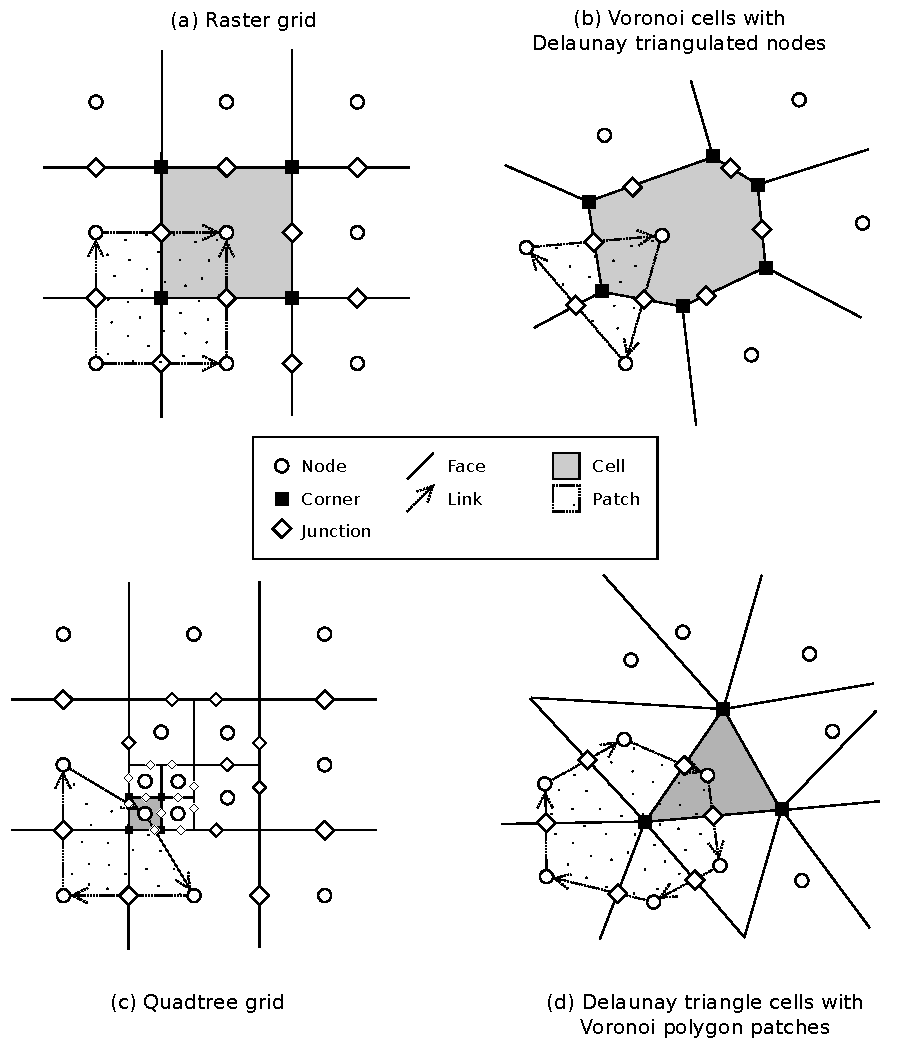
\includegraphics[scale=0.92]{grid_schematic.pdf}
    \caption{Elements of a model grid. Each grid comprises nodes, cells, faces, corners, patches, links, directed edges, and junctions. (Note that not all links, edges, and patches are shown, and only one representative cell is shaded.)}
   \label{grid}
\end{figure}
%%%%%%%%%%%%%%%%%%%%%%%%%%%

Figure~\ref{grid} illustrates how ModelGrid represents a simulation grid. The grid contains a set of $(x,y)$ points called {\em nodes}. In a typical finite-difference model, nodes are the locations at which one tracks scalar state variables, such as water depth, land elevation, or temperature. Each node is associated with a polygon called a {\em cell}. Each cell is bounded by a set of line segments known as {\em faces}, which it shares with its neighboring cells.

In the simple case of a regular (raster) grid, the cells are square, the nodes are the center points of the cells (Figure~\ref{grid}a), and the faces have identical length (equal to the node spacing). In a Voronoi-Delaunay grid, the cells are Voronoi polygons (also known as Theissen polygons) (Figure~\ref{grid}b). In this case, each cell represents the surface area that is closer to its own node than to any other node in the grid. The faces then represent locations that are equidistant between two adjacent nodes. Other grid configurations are possible as well. For examples, cells could be square elements in a quad-tree grid (Figure~\ref{grid}c), or triangular elements with nodes at their circumcenters (Figure~\ref{grid}d).

Each pair of adjacent cells is connected by a line segment called a {\em link} (Figure~\ref{grid}, dashed line). Each link connects a {\em from node} and a {to node}, so it has direction as well as position and length. In some cases, it may be useful to have each pair of adjacent cells connected by two vectors: one pointing one way, and a second pointing the opposite way \citep{guibas1985primitives,tucker2001object}. These vectors are known as {\em directed edges} (Figure~\ref{grid}, gray arrows). 

Finite-difference and finite-volume models usually need to calculate spatial gradients in one or more scalar variables, and often these gradients are evaluated between pairs of adjacent nodes. ModelGrid makes these calculations easier for programmers by providing built-in functions to calculate gradients along links, and allowing applications to associate an array of gradient values with their corresponding links or edges.

The cell vertices are called {\em corners} (Figure~\ref{grid}, solid squares). Each face is therefore a line segment connecting two corners. The intersection of a face and a link (or directed edge) is known as a {\em junction} (Figure~\ref{grid}, open diamonds). Often, it is useful to calculate scalar values (say, ice thickness in a glacier) at nodes, and vector values (say, ice velocity) at junctions. This approach is sometimes referred to as a staggered-grid scheme. It lends itself naturally to finite-volume methods, in which one computes fluxes of mass, momentum, or energy across cell faces, and maintains conservation of mass within cells \citep[e.g.,][]{versteeg2007introduction}.

Notice that the links also enclose a set of polygons that are offset from the cells. These secondary polygons are known as {\em patches} (Figure~\ref{grid}, dotted). This means that any grid comprises two complementary tesselations: one made of cells, and one made of patches. If one of these is a Voronoi tessellation, the other is a Delaunay triangulation. For this reason, Delaunay triangulations and Voronoi diagrams are said to be dual to one another: for any given Delaunay triangulation, there is a unique corresponding Voronoi diagram \citep[e.g.,][]{braun1997modelling,tucker2001object}. With ModelGrid, one can create a mesh with either Voronoi polygons or Delaunay triangles as cells (Figure~\ref{grid}, b and d). Alternatively, with a raster grid, one simply has two sets of square elements that are offset by half the grid spacing (Figure~\ref{grid}a). Whatever the form of the tessellation, ModelGrid keeps track of the geometry and topology of the grid. For example, one can call various ModelGrid functions to obtain lists of the $(x,y)$ coordinates of nodes, corners, and junctions; get lists of neighbors for any cell; get the endpoints of any link or directed edge, and so on. These functions are listed and described below. 

\subsection{How Boundaries are Managed}

An important component of any numerical model is the method for handling boundary conditions. In general, it's up to the application developer to manage boundary conditions for each variable. However, ModelGrid makes this task a bit easier by providing lists of nodes and links that lie along the boundary of the grid, and those that lie in the interior. It also allows you to ``de-activate'' portions of the grid perimeter, so that they effectively act as walls.

Let's look first at how ModelGrid treats its own geometrical boundaries. The outermost elements of a grid are nodes and links (as opposed to corners and faces). For example, Figure~\ref{raster4x5} show a sketch of a regular four-row by five-column grid created by RasterModelGrid. The edges of the grid are composed of nodes and links. Only the inner six nodes have cells around them; the remaining 14 nodes form the perimeter of the grid.

All nodes are tagged as either {\em boundary} or {\em interior}. Those on the perimeter of the grid are automatically tagged as boundary nodes. Nodes on the inside are {\em interior} by default, but it is possible to tag some of them as {\em boundary} instead (this would be useful, for example, if you wanted to represent an irregular region inside a regular grid). In the example shown in Figure~\ref{raster4x5}, all the inner nodes are {\em active interior}, and all perimeter nodes are {\em active boundary}. 

Boundary nodes are flagged as either {\em open (active)} or {\em closed (inactive),} all links are tagged as active or inactive. An {\em active link} is one that joins either two interior nodes, or an  
{\em interior} and an {\em open boundary} node (Figure~\ref{raster4x5openclosed}). You can use this distinction in models to implement closed boundaries by performing flow calculations only on active links. 
Later on, we'll take a look at how this is actually implemented in ModelGrid. Before diving into the nitty-gritty, however, it is useful to walk through an example of how one can use ModelGrid to quickly construct a simple numerical model.


%%%%%%%%%%% FIGURE %%%%%%%%%%%
 \begin{figure}[h!]
    \centering
    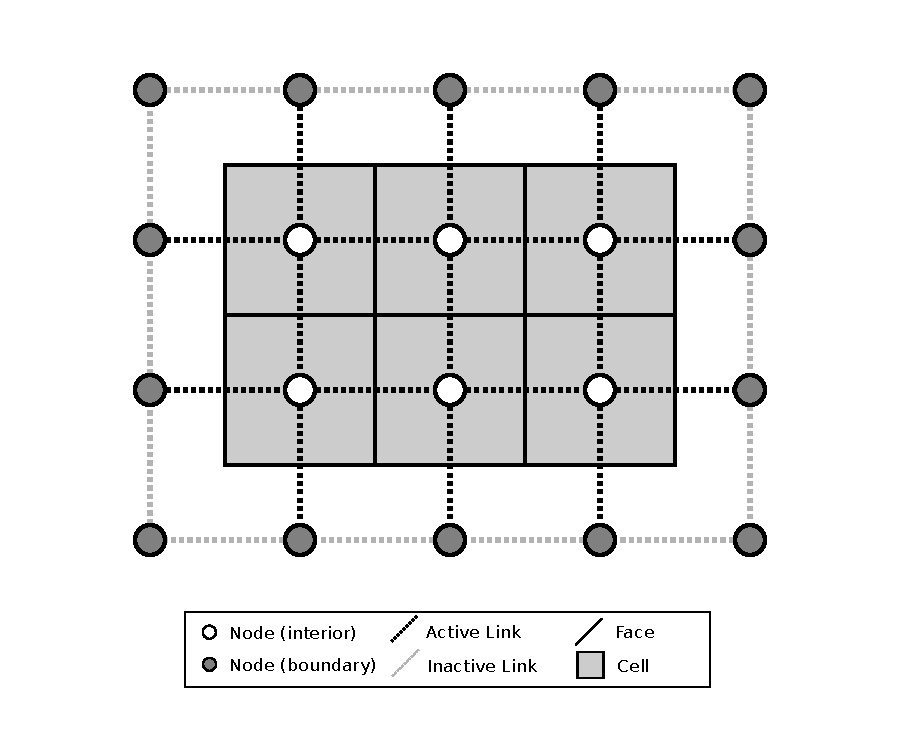
\includegraphics{example_raster_grid.pdf}
    \caption{Illustration of a simple four-row by five-column raster grid created with RasterModelGrid. By default, all perimeter nodes are tagged as active (fixed value) boundaries, and all interior cells are tagged as active interior. An active link is one that connects either two active interior cells, or one active interior and one active boundary.}
   \label{raster4x5}
\end{figure}
%%%%%%%%%%%%%%%%%%%%%%%%%%%

%%%%%%%%%%% FIGURE %%%%%%%%%%%
 \begin{figure}[h!]
    \centering
    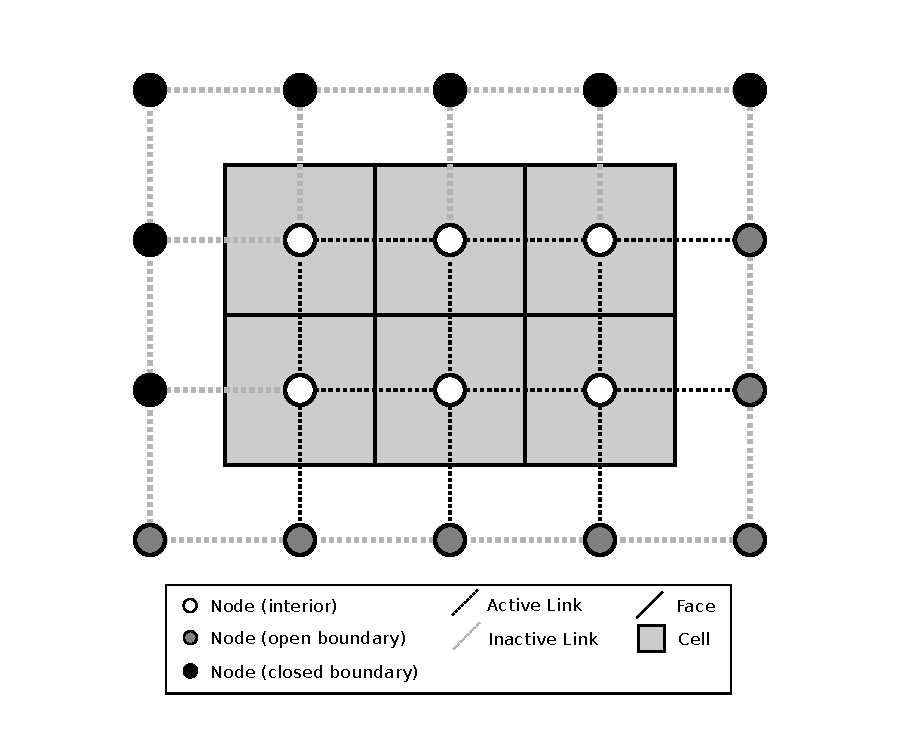
\includegraphics{example_raster_grid_with_closed_boundaries.pdf}
    \caption{Illustration of a simple four-row by five-column raster grid with a combination of open and closed boundaries.}
   \label{raster4x5openclosed}
\end{figure}
%%%%%%%%%%%%%%%%%%%%%%%%%%%



%In ModelGrid, the boundaries of the grid are treated by assigning a {\em boundary code} to each node. The boundary codes are:
%\begin{itemize}
%\item \verb|INTERIOR_NODE|: node is a normal, active interior node.
%\item \verb|FIXED_VALUE_BOUNDARY = 1|: node is meant to have a prescribed value, set by the application. For example, one might maintain a constant elevation, temperature, or ice thickness here.
%\item \verb|FIXED_GRADIENT_BOUNDARY = 2|: indicates that a prescribed gradient is meant to exist between the node and any adjacent interior nodes.
%\item \verb|TRACKS_CELL_BOUNDARY = 3|: indicates that the value at the node is meant to mirror that at another node.
%\item \verb|INACTIVE_BOUNDARY = 4|: indicates that the node is ``inactive,'' meaning that it should not give or receive any flow.
%\end{itemize}
%For the most part, these codes are provided for the convenience of the application developer. The key distinction that ModelGrid actually uses


\section{ModelGrid Example: Diffusion} 

The following is a simple tutorial in which we use ModelGrid to build an explicit, staggered-grid model of diffusion. The mathematics of diffusion describe quite a few different phenomena, among them heat conduction in solids, chemical diffusion of dissolved material, transport of momentum in a viscous shear flow, and transport of soil on hillslopes. To make this exercise concrete, we will use the latter as our working example, though in fact the solution could apply to any of these systems.

To work through this example, you can type in and run the code below, or find a copy at \url{http://csdms.colorado.edu/wiki/Model:LandLab}. The complete source code for the diffusion model is listed below. Line numbers are included to make it easier to refer to particular lines of code (of course, these numbers are not part of the source code). After the listing, we will take a closer look at each piece of the code in turn.

\lstinputlisting[language=Python,caption={diffusion\_with\_model\_grid.py}]{diffusion_with_model_grid.py}



\subsection{Importing Packages}

\begin{lstlisting}[firstnumber=11]
from landlab import model_grid
import pylab
\end{lstlisting}

We start by importing {\tt model\_grid} from the {\tt land lab} package (note that the {\tt landlab} package must first be installed; see instructions XX). We'll also import {\tt pylab} so we can plot the results.


\subsection{Setting the User-Defined Parameters}

\lstinputlisting[firstnumber=14,firstline=14,lastline=29]{diffusion_with_model_grid.py}

The first thing we'll do is set a group of user-defined parameters. The size of the grid is set by \code{numrows} and \code{numcols}, with cell spacing \code{dx}. In this example, we have a 20 by 30 grid with 10~m grid spacing, so our domain represents a 200 by 300~m rectangular patch of land. The diffusivity coefficient \code{kd} describes the efficiency of soil creep, while the \code{uplift\_rate} indicates how fast the land is rising relative to base level along its boundaries. Finally, we set how many time steps we want to compute.

Note that the code for our simple program lives inside a \code{main()} function. This isn't strictly necessary---we could have put the code in the file without a \code{main()} function and it would work just fine when we run it---but it is good Python practice, and will be helpful later on.

\break
\subsection{Calculating Derived Parameters}

\lstinputlisting[firstnumber=31,firstline=31,lastline=33]{diffusion_with_model_grid.py}

Next, we calculate the values of parameters that are derived from the user-defined parameters. In this case, we have just one: the time-step size, which is set by the Courant-Friedrichs-Lewy condition for an explicit, finite-difference solution to the diffusion equation (to be on the safe side, we multiply the ratio $\Delta x^2 / k_d$ by 0.1 instead of the theoretical limit of 1/2). With the parameter values above, $\Delta t = 1000$ years, so our total run duration will be one million years. Remember, though, that the same code could be used for any diffusion application with a source term. For instance, we could model conductive heat flow, with $k_d$ representing thermal diffusivity and \code{uplift\_rate} representing steady head input.


\subsection{Creating and Configuring the Grid}

\lstinputlisting[firstnumber=34,firstline=34,lastline=39]{diffusion_with_model_grid.py}

Our model grid is created with a call to \code{model\_grid.RasterModelGrid()}, which returns a raster model grid object. We then set up this grid with a call to its \code{initialize} method, passing it the desired grid dimensions and spacing.

For our boundary conditions, we would like to keep the nodes along the bottom and right edges of the grid fixed at zero elevation. We also want to have the top and left boundaries represent ridge-lines with a fixed horizontal position and no flow of sediment in or out. To accomplish this, we call the \code{set\_inactive\_boundaries} method on line 39. The method takes four boolean arguments, which indicate whether there should be closed boundary condition on the top, right, bottom, and left sides of the grid. Here we have set the flag to \code{True} for the top and left sides. This means that the links connecting the interior nodes to the perimeter nodes along these two sides will be flagged as inactive, just as illustrated (with a smaller grid) in Figure~\ref{raster4x5openclosed}. As we'll see in a moment, we will simply not bother to calculate any mass flux across these closed boundaries.


\subsection{Creating Data}

\lstinputlisting[firstnumber=41,firstline=41,lastline=50]{diffusion_with_model_grid.py}

Our state variable, $z(x,y,t)$, represents the land surface elevation. One of the unique aspects of ModelGrid is that grid-based variables like $z$ are represented as 1D rather than 2D numpy arrays. Why do it this way, if we have a regular grid that naturally lends itself to 2D arrays? The answer is that we might want to have an irregular, unstructured grid, which is much easier to handle with 1D arrays of values. By using 1D arrays for all types of ModelGrid, we allow the user to switch seamlessly between structured and unstructured grids.

We create our data structure for $z$ values with a call to the \code{create\_node\_dvector} method. The method simply returns a 1D numpy array filled with zeros. The length of the array is equal to the number of nodes in the grid ($20\times 30=600$), which makes sense because we want to have an elevation value associated with every node in the grid.

On the next line, we create a second array, \code{dzdt}, to store the time rate of change of elevation. We only need to calculate $dz/dt$ at the active cells. There are $18\times 28 = 504$ cells, and all of them are active. We create our list of $dz/dt$ values at cells with a call to \code{create\_active\_cell\_dvector}, which creates a numpy array with 504 entries.

When we update elevation values, we will want to operate only on the active cells. To help with this, we obtain an of active cell ID numbers with a call to the \code{get\_interior\_cells} method. Finally, we display a message to tell the user that we're about to run and with what time step size.


\section{Main Loop}

Our model implements a finite-volume solution to the diffusion equation. The idea here is that we calculate sediment fluxes around the perimeter of each cell. We then integrate these fluxes forward in time to calculate the net change in volume, which is divided by the cell's surface area to obtain an equivalent change in height. The numerical solution is given by:
\begin{equation}
\frac{d z_i}{dt} \approx \frac{z^{T+1}_i-z^T_i}{\Delta t}
= - \frac{1}{\Lambda_i} \sum_{j=1}^{N_i} \mathbf{q}_{Sij}^T \lambda_{ij}.
\label{eq:dzdt}
\end{equation}
Here, $z_i^T$ is the elevation at node $i$ at time step $T$, $t$ is time, $\Lambda_i$ is the surface area of cell $i$, $N_i$ is the number of cells adjacent to $i$ (called the cell's {\em neighbors}), $\mathbf{q}_{Sij}^T$ is the sediment flux per unit face width from cell $i$ to cell $j$, and $\lambda_{ij}$ is the width of the face between cells $i$ and $j$. The flux between a pair of adjacent cells is the product of the slope (positive upward) between their associated nodes, $\mathbf{S}_{ij}$, and a transport coefficient, $k_d$,
\begin{equation}
\mathbf{q}_{Sij} = - k_d \mathbf{S}_{ij} = - k_d \frac{z_j-z_i}{L_{ij}}
\end{equation}
where $L_{ij}$ is the length of the link connecting nodes $i$ and $j$. Notice that elevation values (which are scalars) are associated with nodes, while slopes and sediment fluxes (which are vectors) are associated with links and faces. If we want to think of the slopes and fluxes as being calculated at a particular point, that point is the junction between a link and its corresponding face (Figure~\ref{grid}).

\subsection{Calculating gradients and sediment fluxes}

\lstinputlisting[firstnumber=55,firstline=55,lastline=60]{diffusion_with_model_grid.py}

In order to calculate new elevation values, the first quantity we need to know is the gradient (slope) values between all the node pairs. We can calculate this in a single line of code using ModelGrid's \code{calculate\_gradients\_at\_active\_links} method. This method takes a single argument: a 1D numpy array of scalar values associated with nodes. The length of this array must be the same as the number of nodes in the grid. The method calculates the gradients in \code{z} between each pair of nodes. It returns a 1D numpy array, \code{g} (for gradient), the size of which is the same as the number of links in the grid. The sign of each value of \code{g} is positive when the slope runs uphill from a link's {\em from node} to its {\em to node}, and negative otherwise.

To calculate the sediment fluxes, we multiply each gradient value by the transport coefficient \code{kd}. The minus sign simply means that the sediment goes downhill: where the gradient is negative, the flux should be positive, and vice versa. Here, we are taking advantage of numpy's ability to perform mathematical operations on entire arrays in a single line of code, rather than having to write out a \code{for} loop. Line 60 in our code multiplies \code{ks} by every value of \code{g}, and returns the result as a numpy array the same size as \code{g}.

\subsection{Calculating net fluxes in and out of cells}

\lstinputlisting[firstnumber=62,firstline=62,lastline=63]{diffusion_with_model_grid.py}

Now that we know the unit fluxes associated with each link and its corresponding cell face, the next thing we need to do is add up the total flux around the perimeter of each cell. In other words, we need to calculate the summation in equation (\ref{eq:dzdt}). ModelGrid allows us to do this in one line of code, by calling the \code{calculate\_flux\_divergence\_at\_active\_cells} method. This method takes a single argument: a 1D numpy array containing the flux per unit width at each face in the grid. The method multiplies each unit flux by its corresponding face width, adds up the fluxes across each face for each cell, and divides the result by the surface area of the cell. It returns a 1D numpy array that contains the net rate of change of volume per unit cell area. The length of this array is the same as the number of cells in the grid. Note, though, that the returned value will be zero for any and all boundary cells. In our diffusion example, we will store the result in \code{dqsds}.

\subsection{Updating elevations}

\lstinputlisting[firstnumber=65,firstline=65,lastline=70]{diffusion_with_model_grid.py}

When we calculated flux divergence, we got back an array of numbers, \code{dasds}, that represent the deposition (positive) or erosion (negative) rate of each cell. Now we need to combine this with the source term---representing rock uplift relative to the base level at the model's fixed boundaries---in order to calculate the total rate of elevation change at the nodes. We don't want to apply this calculation to the boundary cells, however. We therefore use a \code{for} loop to calculate the rate of elevation change \code{dzdt} at only the interior cells. Once we've calculated rates of change, we update all node elevations by simply multiplying \code{dzdt} by our time step size. (Note that we could have combined the calculation of rates of change and updating of new elevations into a single line; this would slightly improve performance, but the code would be less clear).

\subsection{Updating no-flux boundaries}

\lstinputlisting[firstnumber=72,firstline=72,lastline=73]{diffusion_with_model_grid.py}

The last step in the loop is to update any zero-gradient (no-flux) boundaries. The call to \code{update\_noflux\_boundaries} simply sets the elevation of any no-flux boundary nodes to the elevation of the adjacent interior neighbor. This way, the gradient and hence the flux will be zero at that interface.


\section{Plotting the Result}

\lstinputlisting[firstnumber=78,firstline=78,lastline=95]{diffusion_with_model_grid.py}

The last section of the \code{main} function plots the result of our calculation. We do this using pylab's \code{imshow} and \code{contour} functions to create a colored image of topography overlain by contours. To use these functions, we need our elevations to be ordered in a 2D array. We obtain a 2D array version of our \code{z} values through a call to RasterModelGrid's \code{cell\_vector\_to\_raster} method.

The last two lines of code are standard Python syntax. They will execute the \code{main} function when the code is run, but not when the code is simply imported as a module.


 
\newpage
\bibliography{/Users/gtucker/Documents/Literature/gt_library.bib}
\bibliographystyle{/Users/gtucker/Documents/Literature/agufull08}



\end{document}